\section{Vztahy mezi goniometrickými funkcemi}
\begin{pozn}
    Věty \ref{soucsc} a \ref{dvojnas}
    musíme umět nazpaměť.
\end{pozn}

\begin{veta}[Součtové vzorce]\label{soucsc}
    $\forall x, y \in \mathbb{R}: $
    \begin{align*}
        \sin \left(x\pm y\right) & = \sin x \cdot \cos y \pm \cos x \cdot \sin y, \\
        \cos \left(x\pm y\right) & = \cos x \cdot \cos y \mp \sin x \cdot \sin y.
    \end{align*}
\end{veta}

\begin{proof}
    Nechť jsou dány dva vektory $\vec u=(\cos \alpha, \sin \alpha), \vec v = (\sin \beta, \cos \beta), \alpha, \beta \in \left( 0,\frac{\pi}{2} \right ) $,
    tedy vektor $\vec u$ svírá s $x$-ovou osou úhel $\alpha$ a vektor $\vec v$ svírá s
    $y$-ovou osou úhel $\beta$. Označme orientovaný úhel, který svírají vektory $\vec u,\vec v$
    jako $\varphi$.
    \begin{figure}[h!]
        \centering
        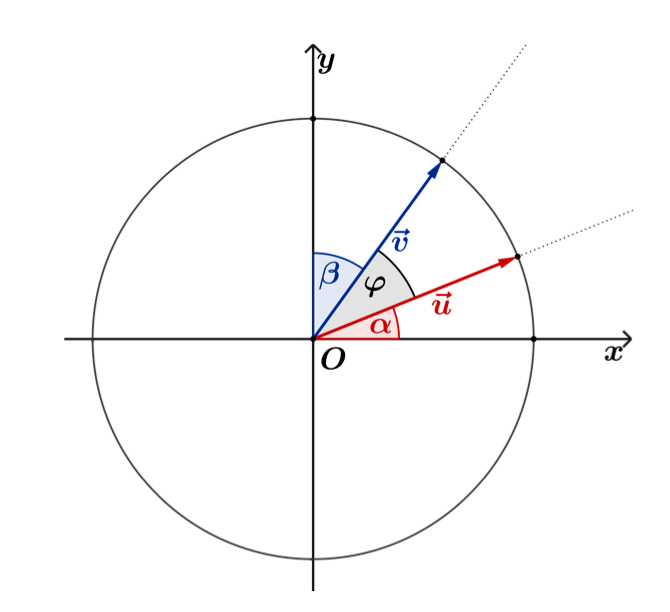
\includegraphics[width=0.25\textwidth]{souctove_vzorce.png}
    \end{figure}
    Platí tedy $\alpha+\beta+\varphi=\frac{\pi}{2}\implies \varphi = \frac{\pi}{2}-(\alpha+\beta)$.
    Obecně platí $\cos \theta = \sin \left ( \frac{\pi}{2}-\theta \right ) $, v našem
    případě $\cos \varphi=\sin (\alpha+\beta).$ Úhel $\varphi$ lze spočítat pomocí
    součinu
    $$\cos \varphi = \frac{\vec u\cdot \vec v}{|\vec u|\cdot |\vec v|}=\cos \alpha \sin \beta + \sin \alpha \cos \beta, \textrm{ neboť } |\vec u| = |\vec v| = 1.$$
    Celkem tedy máme
    $$\sin (\alpha+\beta) = \cos \varphi = \sin \alpha \cos \beta+\cos \alpha \sin \beta,$$
    což jsme chtěli dokázat. Pro ostatní případy analogicky.
\end{proof}

\begin{veta}\label{dvojnas}
    $ \forall x \in \mathbb{R}:$
    \begin{align*}
        \sin 2x = 2\sin x \cdot \cos x, & & \cos 2x = \cos^2 x - \sin^2 x.
    \end{align*}
\end{veta}

\begin{proof}
    Plyne jednoduše z věty \ref{soucsc}.
\end{proof}

\begin{pozn}
    Následující vztahy stačí \uv{rychle odvodit}.
\end{pozn}

\begin{veta}[Vyjádření gon. funkce pomocí jiné gon. funkce]\label{vyjadrenigonf}
  \,\\
  \begin{tabular}{| c || c | c | c | c |}
    \hline
    & $\sin x$ & $\cos x$ & $\tg x$ & $\cotg x$ \\
    \hline\hline
    $\sin x$ & -- & $\sqrt{1-\cos^2 x}$ & $\frac{\tg x}{\sqrt{1+\tg^2 x}}$ & $\frac{1}{\sqrt{1+\cotg^2 x}}$\\
    \hline
    $\cos x$ & $\sqrt{1-\sin^2 x}$ & -- & $\frac{1}{\sqrt{1+\tg^2 x}}$ & $\frac{\cotg x}{\sqrt{1+\cotg^2 x}}$\\
    \hline
    $\tg x$ & $\frac{\sin x}{\sqrt{1-\sin^2 x}}$ &  $\frac{\sqrt{1-\cos^2 x}}{\cos x}$ & -- & $\frac{1}{\cotg x}$\\
    \hline
    $\cotg x$ & $\frac{\sqrt{1-\sin^2 x}}{\sin x}$ & $\frac{\cos x}{\sqrt{1-\cos^2 x}}$ & $\frac{1}{\tg x}$ & --\\
    \hline
  \end{tabular}

\end{veta}



\begin{proof}
    Pro druhý až čtvrtý kvadrant v tabulce plyne z definice. \\
    Vyjádření sinu nebo kosinu pomocí funkce tangens nebo kotangens nalezneme
    jednoduše ze vztahů v pravoúhlém trojúhelníku. Nechť je dán pravoúhlý trojúhelník
    s přeponou $b.$ Pak $\tg \alpha = \frac{a}{c},$ položme tedy $a = \tg \alpha$ a $c=1. $
    Potom z Pythagorovy věty plyne $b=\sqrt{1+\tg^2 \alpha}. $ Pak $\sin\alpha = \frac{\tg x}{\sqrt{\tg^2 x+1} }$ a
    $\cos \alpha = \frac{1}{\sqrt{\tg^2 \alpha + 1} }.$ Obdobně i pro kotangens.
\end{proof}

\begin{priklad}
Určete hodnoty všech goniometrických funkcí, je-li dáno $\sin x=\frac{1}{3}, x \in \left ( \frac{\pi}{2},\pi \right ). $
\end{priklad}

\begin{reseni}
Podle vztahů ve větě \ref{vyjadrenigonf}.
\end{reseni}

\begin{priklad}
Vypočtěte hodnoty všech goniometrických funkcí v bodě $\alpha = 105^\circ$.
\end{priklad}

\begin{reseni}
Využijeme toho, že $105=60+45,$ což jsou tabulkové hodnoty, a součtových vzorců.
\end{reseni}

\begin{veta}
  $\forall x,y, (x\pm y)\in\mathbb{R}\smallsetminus\bigcup\limits_{k\in\mathbb{Z}} \left\{\frac{(2k+1)\pi}{2}\right\}:$
  $$\tg\left(x\pm y\right) = \frac{\tg x \pm \tg y}{1\mp\tg x \cdot \tg y}.$$
\end{veta}
\begin{proof}
    Počítejme:
    \begin{align*}
        \tg \left(x+y\right) & = \frac{\sin \left(x+y\right)}{\cos \left(x+y\right)}=\frac{\sin x\cdot  \cos y + \cos x\cdot  \sin y}{\cos x \cdot \cos y - \sin x\cdot  \sin y} \\
        & = \frac{\frac{\sin x \cdot \cos y + \cos x\cdot  \sin y}{\cos x \cdot \cos y}}{\frac{\cos x\cdot  \cos y - \sin x \cdot \sin y}{\cos x\cdot  \cos y}}=\frac{\tg x + \tg y}{1-\tg x \cdot \tg y}.\qedhere
    \end{align*}
\end{proof}


\begin{veta}
  $\forall x,y,(x\pm y)\in\mathbb{R}\smallsetminus\bigcup\limits_{k\in\mathbb{Z}} \left\{\frac{k\pi}{2}\right\}:$
  $$\cotg\left(x\pm y\right) = \frac{\cotg x \cdot \cotg y \mp 1}{\cotg x \pm \cotg y}.$$
\end{veta}

\begin{proof}
    Počítejme:
    \begin{align*}
        \cotg \left(x+y\right) & = \frac{\cos \left(x+y\right)}{\sin \left(x+y\right)}=\frac{\cos x \cdot \cos y - \sin x\cdot  \sin y}{\sin x\cdot  \cos y + \cos x\cdot  \sin y}\\
       &  = \frac{\frac{\cos x\cdot  \cos y - \sin x \cdot \sin y}{\sin x \cdot \sin y}}{\frac{\sin x \cdot \cos y + \cos x\cdot  \sin y}{\sin x\cdot  \sin y}}=\frac{\cotg x \cdot \cotg y-1}{\cotg x + \cotg y}.\qedhere
    \end{align*}
\end{proof}

\begin{veta}
    $\forall x \in \mathbb{R}:$
    \begin{align*}
        \left| \sin \frac{x}{2} \right| = \sqrt{\frac{1-\cos x}{2}}, & & \left| \cos \frac{x}{2}\right| = \sqrt{\frac{1+\cos x}{2}}.
    \end{align*}
\end{veta}

\begin{proof}
  $\cos^2 \frac{x}{2} - \sin^2 \frac{x}{2} = \cos x$ a
  $\cos^2 \frac{x}{2} + \sin^2 \frac{x}{2} =1 $
  \begin{align*}
    2\cos^2 \frac{x}{2}&=\cos x +1 & 2\sin^2 \frac{x}{2} & =1-\cos x \\
    \cos^2 \frac{x}{2}&=\frac{\cos x +1}{2} & \sin^2 \frac{x}{2} & =\frac{1-\cos x }{2} \\
    \left| \cos \frac{x}{2} \right| &= \sqrt{\frac{\cos x +1}{2}} & \left| \sin \frac{x}{2} \right | & = \sqrt{\frac{1-\cos x}{2}}\qedhere
  \end{align*}
\end{proof}

\begin{veta}
  $\forall x,y \in \mathbb{R}:$
  \begin{align*}
    \sin x + \sin y &= 2\sin \frac{x+y}{2}\cdot \cos \frac{x-y}{2},& & \cos x + \cos y = 2 \cos \frac{x + y}{2}\cdot \cos \frac{x - y}{2},\\
    \sin x - \sin y &= 2\cos \frac{x + y}{2}\cdot \sin \frac{x - y}{2},& & \cos x - \cos y =-2\sin \frac{x + y}{2}\cdot \sin \frac{x -y}{2}.
  \end{align*}
\end{veta}

\begin{proof}
    Počítejme:
    \begin{align*}
        \sin x + \sin y & = \sin \left(\frac{x+y}{2}+\frac{x-y}{2}\right)+ \sin \left(\frac{x+y}{2}-\frac{x-y}{2}\right ) \\
        & = \sin \frac{x+y}{2} \cos\frac{x-y}{2} + \cos\frac{x+y}{2} \sin \frac{x-y}{2} \\
        & + \sin \frac{x+y}{2} \cos\frac{x-y}{2} -  \cos\frac{x+y}{2} \sin \frac{x-y}{2}\\
        & = 2\sin \frac{x+y}{2} \cos\frac{x-y}{2}.
    \end{align*}
  V ostatních případech analogicky.
\end{proof}

\begin{priklad}
Vyjádřete jako součin: $\sin 3y+\sin y.$
\end{priklad}

\begin{reseni}
Platí
$\sin 3y+\sin y=2\sin \frac{3y+y}{2}\cdot \cos \frac{3y-y}{2}=2\sin 2y \cdot \cos y.$
\end{reseni}

\begin{veta}[Sinová věta]
    V každém trojúhelníku $ABC$ platí
    $$\frac{a}{\sin \alpha} = \frac{b}{\sin \beta}=\frac{c}{\sin \gamma}=2R,$$
    kde $R$ je poloměr kružnice opsané.
\end{veta}

\begin{veta}[Kosinová věta]
 V každém trojúhelníku $ABC$ platí
 \begin{align*}
    a^2 &= b^2+c^2-2bc\cos \alpha, \\
    b^2 &= a^2+c^2-2ac\cos \beta ,\\
    c^2 &= a^2+b^2-2ab\cos \gamma.
 \end{align*}
\end{veta}

\begin{veta}\label{obsahtroj}
     V každém trojúhelníku $ABC$ platí
     $$\frac{abc}{4R}=S=\rho s,$$
     kde $R$ je poloměr kružnice opsané a $\rho$ poloměr kružnice vepsané.
\end{veta}

\begin{veta}[Heronův vzorec]
    V každém trojúhelníku $ABC$ platí
    $$S=\sqrt{s(s-a)(s-b)(s-c)}, $$
    kde $s$ je polovina obvodu.
\end{veta}

\begin{priklad}
Nalezněte vztah mezi poloměrem kružnice vepsané a opsané trojúhelníku $ABC$.
\end{priklad}

\begin{reseni}
Zjistíme jednoduše z věty \ref{obsahtroj}.
\end{reseni}

\begin{priklad}
Vrchol věžě stojící na rovině vidíme z místa $A$ pod výškovým úhlem $\alpha= 39^\circ 28^\prime$.
Přijdeme-li o 50 metrů blíž, je vidět pod úhlem $\beta=58^\circ 42^\prime.$ Jak vysoká je věž?
\end{priklad}

\begin{reseni}
Použitím sinové a kosinové věty.
\end{reseni}
